
%Works on MiKTeX only
%hint by http://goemonx.blogspot.de/2012/01/pdflatex-ligaturen-und-copynpaste.html
%also http://tex.stackexchange.com/questions/4397/make-ligatures-in-linux-libertine-copyable-and-searchable
%This allows a copy'n'paste of the text from the paper
\input glyphtounicode.tex
\pdfgentounicode=1

This section provides an overview of same major contributions in this area. Section 2.1 provides an insight about the core concepts of cloud computing, such as the architectural and business models of cloud computing. Section 2.2 describes some open standards related to the authentication and authorization protocols. Finally, Section 2.3 provides a comparison between the most known cloud storage providers and their services, including features and prices.
\subsection{Cloud Computing Core Concepts}\label{ssec:tools}
%%%%%%%%%%%%%%%%%%%%%%%%%%%%%%%%%%%%%%%%%%%%%%%%%%%%%%%%%%%%%%%%%%%%%%%%%%%%%%%

Described by the National Institute of Standards and Technology (NIST) as a {\it model for enabling convenient, on-demand network access to a shared pool of configurable computing resouces (e.g., networks, servers, storage, applications, and services) that can be rapidly provisioned and released with minimal management effort or service provider interaction}, \cite{Zhang2010}
cloud provides an architecture that can be divided into 4 layers: the hardware layer, the infrastructure layer, the platform and the application layer, as described bellow:

\begin{itemize}
\item \textit{The hardware layer}\\
Typically implemented in data centers, is responsible for managing the physical resources of the cloud, such as physical servers, routers, switches, power and cooling systems. Typical issues at hardware layer include hardware configuration, fault tolerance and traffic and power management.\cite{cloud:SS}\\

\item \textit{The infrastructure layer}\\
The infrastructure layer creates a pool of storage and computing resources by partitioning the physical resources using virtualization technologies (e.g., KVM, Xen, VMWare). It is an essential component of cloud computing since may key features are only available through virtualization technologies.\cite{cloud:SS} \\

\item \textit{The platform layer}\\
The platform layer is composed of the operating systems and application frameworks. Built on top of the infrastructure layer, the platform tries to minimize the load of deploying applications directly into VM containers. One of the best examples is the Google App Engine that operates at the platform layer to provide API support for implementing storage, database and business logic of typical web applications.\cite{cloud:SS}\\

\item \textit{The application layer}\\
Located at the the highest level of the hierarchy, the application layer consists of the actual cloud applications that make use of automatic-scaling feature to achieve better performance, availability and lower operating cost.\cite{cloud:SS}
\end{itemize}

Cloud computing also employs a service business model where hardware and platform-level resources are provided as services on-demand. In fact, every layer describe in the architecture can be implemented as a service to the layer below. Due to this fact, cloud offers services  that can be assigned to each layer, and grouped into three categories: infrastructure as a service (IaaS), platform as a service (PaaS) and software as a service (SaaS).


\begin{itemize}
\item \textit{IaaS - Infrastructure as a Servive }\\
It refers to on-demand provisioning of infrastructural resources i.e. users can subscribe to their favorite computing infrastructures with specified requirements in terms of hardware configuration, software installation and data access. Examples of IaaS providers include Amazon EC2 \cite{iaas:AmazonEC2} , GoGrid \cite{iaas:GoGrid} and Flexiscale\cite{iaas:FlexiScale}.  \\


\begin{figure}[h]
    \centering
    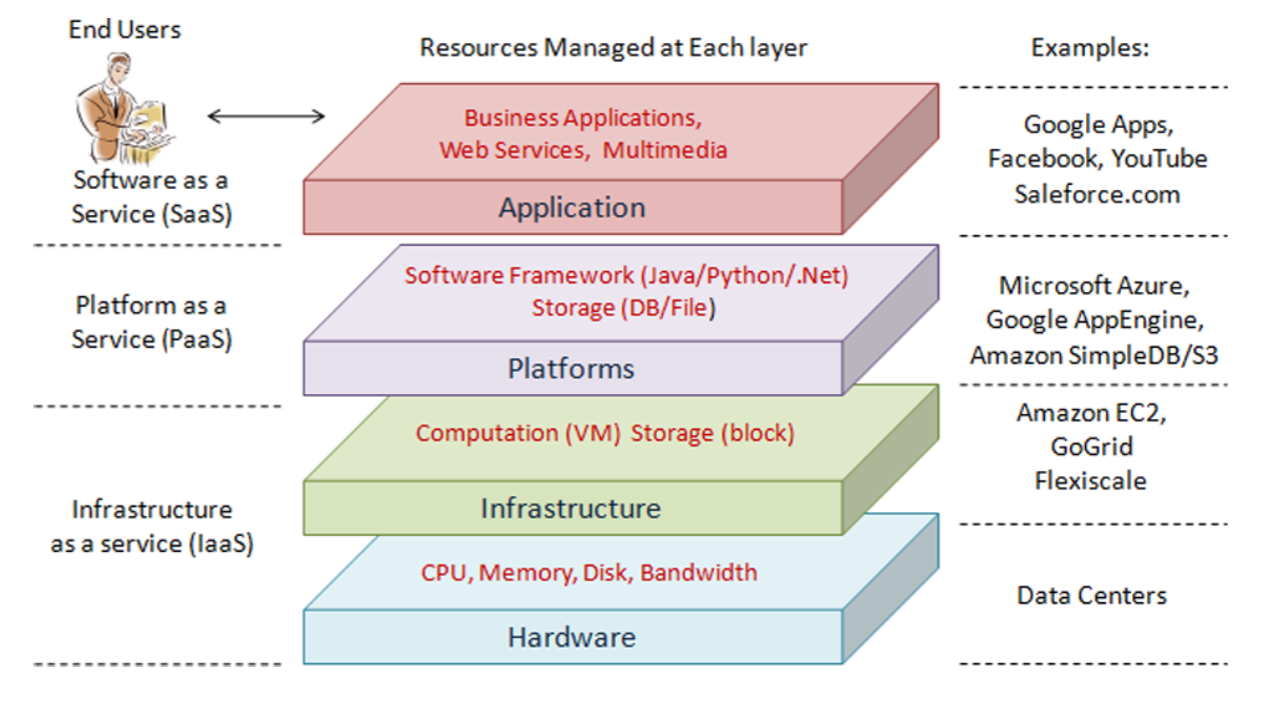
\includegraphics[width=\textwidth]{cloudArchitecture}
    \caption{Cloud Computing Architecture \cite{cloud:Archi}}
    \label{fig:cloudArchitecture}
\end{figure}

\item \textit{PaaS - Platform as a Servive }\\
It refers to the provisioning of platform software layer resources, including operating system support and software development frameworks. Examples of PaaS providers include Google App Engine, Microsoft Windows Azure and Force.com \cite{paas:Force}.\\

\item \textit{SaaS - Software as a Servive }\\
Software or an application is hosted as a service and provided to customers over the Internet. This is a very important service since it eliminates the need to install and run the application on the local computer. An important example of the SaaS is the Application Service Provider (ASP) whose main approach is to provide subscriptions to software that is hosted in the Internet. Google Chrome Browser is another example since it provides a desktop through which applications can be delivered locally or remotely, in addition to the traditional web browsing experience. Another examples include SalesForce.com and Rackspace \cite{saas:RackSpace}\\
\end{itemize}


\subsection{Web Authentication \& Authorization Open Technology}\label{ssec:security}


\begin{itemize}
\item {\it OpenID -} is an open standard for user authentication that allows the use of an existing account to sign in to multiple websites, without needing to create new passwords. It offers the possibility to associate information ( such as name or email address) with user's OpenID, that can be shared with the websites visited.

\begin{figure}[h]
    \centering
    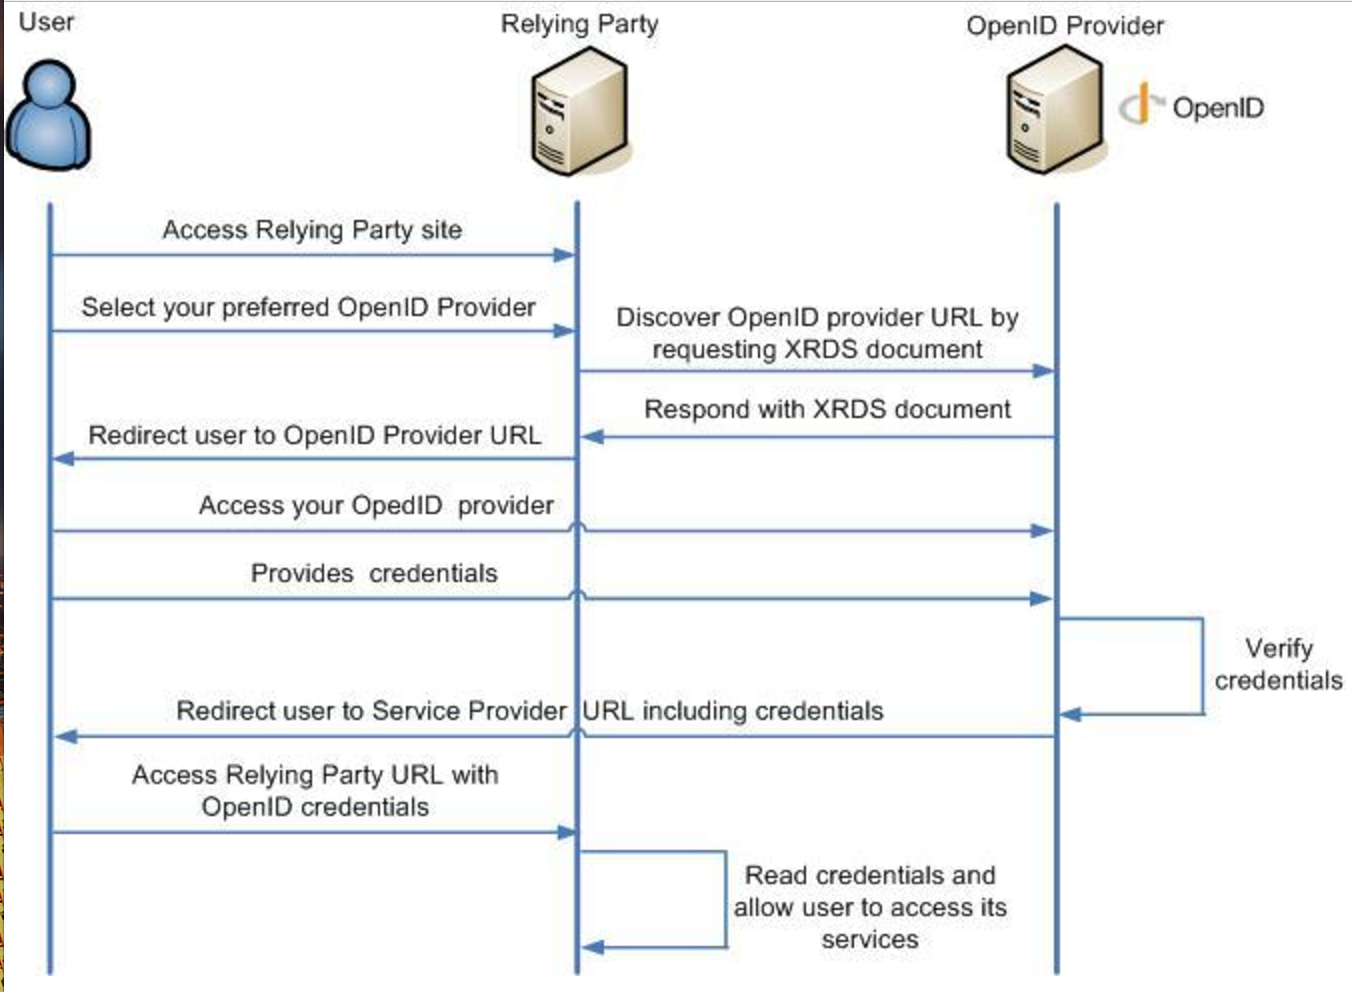
\includegraphics[width=1.0\textwidth]{openID}
    \caption{OpenID Authentication Flow}
    \label{fig:openID}
\end{figure}
%(citar o openID http://openid.net/get-an-openid/what-is-openid/).
To do that OpenID provides a framework for communication between the identity provider and the relying party. The user may have an account or multiple accounts with a specified identity provider, and then use this identity to authenticate to any service that accepts OpenID authentication. 

The flow process of OpenID comprises three entities: the user, the relying party which wants to verify the user identity and an entity provider that provides the OpenID URLs as despicted in figure \ref{fig:openID}.\\

With OpenID the user's password is only given to the identity provider and this one confirms the identity to the websites visited so, no website sees the password. Therefore, it is considered as safe since it not compromises the user's identity by some kind of insecure websites.\cite{cloud:openID}\\


\item {\it Shibboleth -} is another open standard, similar to OpenID, whose main approach is to manage single sign on (SSO), allowing users to authenticate to different services using just one piece of information.
Shibboleth is an open source implementation of federated identity based management, where the identity providers provide information and the service providers consume this information giving access to content or services. %{\textbf CITAR https://shibboleth.net/about/}. 

A user authenticates with his organizational credentials, and the organization (or identity provider) passes the minimal identity information necessary to the service provider to enable an authorization decision. It also provides extended privacy functionality allowing a user to control the attributes released to each application.\\ %{\textbf CITAR 15\\}


\item {\it OAuth - } is an open standard that provides a solution for internet users to authorize websites or applications to access their information, without sharing their credentials such as passwords or usernames.%\textbf {CITAR: Whitson Gordon. "Understanding OAuth: What Happens When You Log Into a Site with Google, Twitter, or Facebook". Retrieved 2016-05-15.}
Designed to work specifically with Hypertext Transfer Protocol (HTTP), it allows access tokens to be issued to third-party clients by an authorization server, with the approval of the resource owner. The third party then uses the access token to access the protected resources hosted by the resource server. %\textbf{CITAR: "RFC 6749 - The OAuth 2.0 Authorization Framework". Retrieved 2016-05-15.}

\begin{figure}[h]
    \centering
    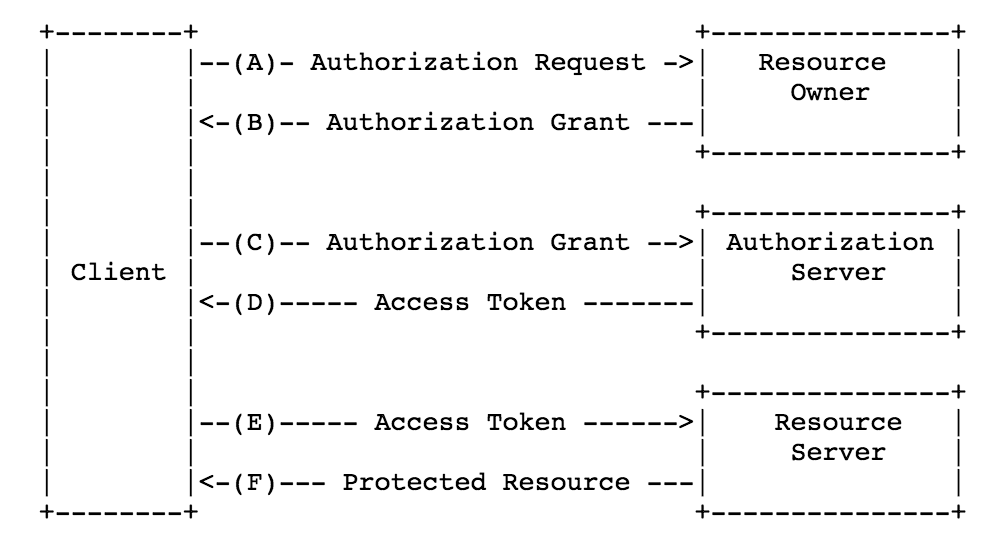
\includegraphics[width=1.0\textwidth]{OAuth}
    \caption{OAuth Protocol flow}
    \label{fig:OAuth}
\end{figure}

Since the creation, OAuth is being used by many social networking websites for authorization of various applications. Once the permissions are granted the application is able to download the complete stream of social data agains the user which is then kept for data mining purposes.% \textbf{CITAR O PAPER}.
More than a protocol, it is a framework is interoperable with any newer version of itself (e.g. Auth2.0).   
\end{itemize}

\subsection{Cloud Providers}\label{ssec:storage}

The industry of cloud storage has lot of potential in terms of growth of storage and faster retrieval. When organizations call for certain services offered by Cloud Storage Providers (CSPs), it is implicit that the they will choose the CSP that best suits the requirements of such organization. CSPs are also defined as Hosts, responsible for keeping the data available and accessible in a physical environment protected and running. People and organizations buy or lease storage capacity from the storage provider in order to store user, organization, or application data. Cloud storage Services may be accessed through cloud computer service, a web service application programming interface (API) or by applications that utilize the API, such as cloud desktop storage, a cloud storage gateway \cite{cloud:cloudStorageGateway} or Web-based content management systems.

Many cloud storage services offers a free account with some limitations, such as the amount of storage provided (usually from 2GB up to 5GB), or a file size limit for upload. 
An overview of the services  of the dominant Cloud Providers in the industry and their services is given bellow. 

\begin{enumerate}
\item {\it Amazon Cloud Drive -}
Amazon Cloud Drive is a cloud storage application managed by Amazon that offers secure cloud storage, file backup, file sharing and photo printing. Acting like a personal hard drive in the cloud, it can be accessed through multiple devices and offers 2 types of plans: one enables user with an unlimited storage for photos and the other one offers a 5GB of cloud storage space free of cost in a three-month trial.
There is no limit for the number of files to be uploaded, but each file needs to be under 2GB.

The advantage of Amazon Cloud Drive resides on the fact that if the user already have an Amazon account, doesn't need to sign up for a new service.
However, unlike other cloud storage services, the desktop app just allows the user to upload or download files, and can only view or manage files from the cloud drive website.\\

\item {\it Dropbox -}
Dropbox is one of the most used cloud storage services, allowing the store of any kind of file in the cloud. With Dropbox, users can easily move files from their computers to the cloud and vice versa by dragging and dropping them into the Dropbox folder.
The service automatically and quickly syncs files across all the devices registered for a specified account, available everywhere and independent from the device that it is being used. 
There is no size limit on file upload, but larger files can take several hours to upload, depending on network connection speed.
As an advantage, Dropbox gives its users a lot of opportunities to get extra storage (despite the 2GB offered through the sign up). If the user participate in the quick Getting Started Tutorial, the space increases more 250MB. Turn on the automatic photo upload feature on any of the mobile apps allows more 3GB of extra space. It's also possible to earn 500MB for each friend referred to Dropbox if it actually signs up for the service, up to 16GB total, or 32 referrals.
However, the website does not allow user to control how files are displayed.\\

\item {\it Box -}
Box is another cloud storage service that also provides sharing and privacy features for business and users. Beyond the basic cloud storage setup, where it's possible to store any kind of file, Box lets users to share files between them, assign tasks, leave comments on someone's work and get notifications when a file changes. User can also preview files from Box website and even create simple text documents. Like other cloud storage services box gives a lot of control over the privacy of a file, allowing user to decide who can view and open specific folders and files. It also allows user to define passwords for his files and set expiration dates for shared folders.
One of biggest advantages of Box is that, it allows business users to connect 
other apps, such as Salesforce and NetSuite \cite{cloud:netSuite}, so that you can easily save documents to Box. There are also plug-ins for Microsoft Office and Adobe Lightroom that let the user open and edit files saved to Box from those applications.

However The service's endless list of sharing and privacy features can be lost on someone who's just using the service for personal storage.
Because of all those features, it can feel overwhelming to navigate the Box website if you're only trying to manage a few files and folders.\\

\item {\it Microsoft OneDrive -}
OneDrive is a cloud storage service provided by Microsoft, that allows the store of any kind of file in the service, including photos, video and documents, and then access them from any Windows desktop or mobile device. One of the most important strengths of OneDrive, is that it works closely with Microsoft Office apps (e.g. Office 365). Therefore, anyone that has an Office 365 subscription will have access to OneDrive, collaborating with other people in real time.

In late 2015, Microsoft made an announcement that it would no longer offer unlimited cloud storage to Office 365 subscribers. Instead, subscribers are limited to 1TB. In the case of OneDrive Storage plans it offers a 50GB for \$1.99 per month plan (besides the 5GB offered initially to anyone that has a Microsoft Account). 
Another disadvantage of OneDrive resides on the fact that, the automatic file organization not always put files in the correct folders.\\

\item {\it Google Drive -}
Google Drive is the cloud storage service created by Google. Released on April 2012, allows users to store files in the cloud, synchronize files across devices and share files. It also combines a complete set of office tools such Google Docs, Sheets and Slides in an office suite that provides collaborative editing of documents, spreadsheets and presentations.
For those who have a Google account, it's easy to access google drive and enable the service in seconds. However, the 15GB initially provided are shared with other services such as Gmail (it's possible to save attachments from the e-mail directly to drive), and Google+. Like the other cloud providers, google drive can be accessed through a web browser or desktop app, but unfortunately if the user uses Google Drive tools to create documents, spreadsheets or presents, it must export those files to edit them in another program.
\end{enumerate}
The following table provides an overview of all the cloud providers described above and makes a comparison between them in terms of file size restriction, free storage, the possibility of earn extra storage, the paid plans that are available in the market and specific costs and the operative systems that supports each kind of service.
\begin{center}
\begin{tabular}{ |M{2.5cm}|M{2cm}|M{2cm}|M{2cm}|M{2cm}|M{2cm}|M{2cm}| }
 \hline
 \multicolumn{6}{|c|}{\textbf{Cloud Providers Comparison}} \\
 \hline
 & \textbf{OneDrive} & \textbf{Dropbox} & \textbf{Google Drive} & \textbf{Box} & \textbf{Amazon Cloud Drive}\\
 \hline
 \textbf{File Size Restriction} & 10GB&10GB with website, none with Dropbox apps&5TB&250MB for free plan, 5GB for paid personal plan&2GB*\\  \hline
 \textbf{Free storage} & 5GB&2GB&15GB&10GB&No**\\  \hline
 \textbf{Earn extra free storage} & No & Yes & No & No & No\\ \hline
 \textbf{Paid Plans} & €2/month for 50GB & €8.25/month for 1TB, €10/month unlimited storage for business teams (each user)	& €2/month 100GB, €10/month for 1TB up to 30TB of storage & €10/month for 100GB & €10.99/year for unlimited photos, €60/year for unlimited storage\\ \hline
 \textbf{OSes supported}	 & Windows, Mac, Android, iOS, Windows Phone	& Windows, Mac, Linux, Android, iOS, Windows Phone, BlackBerry, Kindle Fire	&Windows, Mac, Android, iOS	&Windows, Mac, Android, iOS, Windows Phone, BlackBerry	& Windows, Mac, Android, iOS, Kindle Fire.
\\
 \hline
\end{tabular}
*There is no file size limit with desktop apps.\\
**Amazon Cloud Drive offers limited free storage with an Amazon Prime subscription.
\end{center}



